\documentclass{article}
\usepackage[UTF8]{ctex}
\usepackage{amsmath}
\usepackage{amssymb}
\usepackage{graphicx}
\usepackage{geometry}
\geometry{a4paper, margin=2cm}

\newcommand{\problemname}[1]{\begin{center}\Large\bfseries #1\end{center}}
\usepackage{enumitem}

\begin{document}
\problemname{日历}

在西洋历中，周日是每周的第一天，下面是某年 $11$ 月份的日历：

\begin{center}
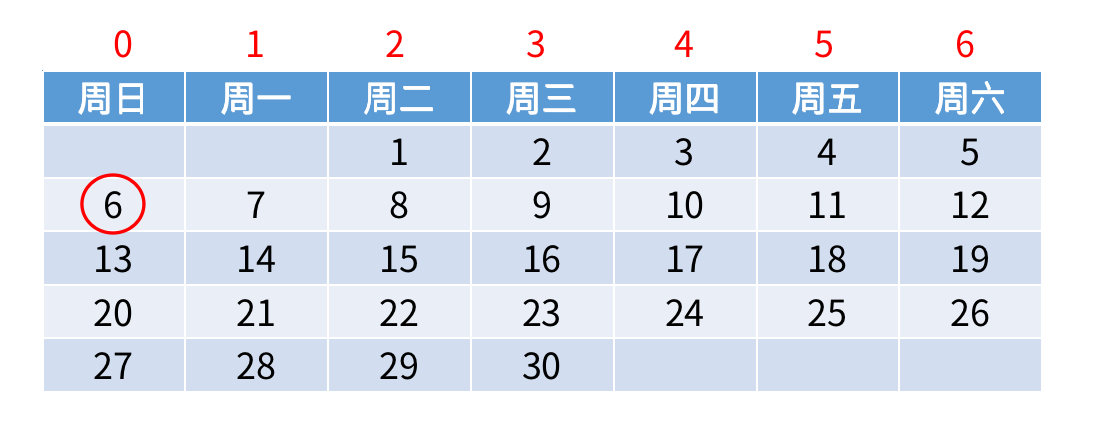
\includegraphics[width=0.7\textwidth]{suanfa35927-f8036b0ade92906cdf9c.png}
\end{center}

现在使用 $0$ 表示周日，使用 $1\sim6$ 表示周一到周六。

已知今天是 $11$ 月 $6$ 日，周日（使用数字 $0$ 表示）。

蒜头君想要知道 $n$ 天后，是周几？

\subsection*{输入格式}
输入一个整数 $n(0<n<100)$，表示天数。

\subsection*{输出格式}
输出一个整数，表示 $n$ 天后是周几。

\begin{itemize}
  \item 如果 $n$ 天后是周日，则输出 \texttt{0}；

  \item 如果 $n$ 天后是周一，则输出 \texttt{1}；

  \item 如果 $n$ 天后是周二，则输出 \texttt{2}；

  \item 如果 $n$ 天后是周三，则输出 \texttt{3}；

  \item 如果 $n$ 天后是周四，则输出 \texttt{4}；

  \item 如果 $n$ 天后是周五，则输出 \texttt{5}；

  \item 如果 $n$ 天后是周六，则输出 \texttt{6}；

\end{itemize}
\subsection*{样例输入}
\begin{verbatim}
2
\end{verbatim}

\subsection*{样例输出}
\begin{verbatim}
2
\end{verbatim}

$2$ 天后是 $11$ 月 $8$ 日，周二。

\subsection*{样例 2 输入}
\begin{verbatim}
10
\end{verbatim}

\subsection*{样例输出}
\begin{verbatim}
3
\end{verbatim}

$10$ 天后是 $11$ 月 $16$ 日，周三。


\end{document}
